\clearpage

\section{Vista Física}

\subsection{Topología compartida}

La \textbf{topología del sistema} se define a partir de los distintos pipelines necesarios para resolver cada consulta. Todas las consultas comparten una sección común formada por tres componentes principales.

\textbf{Servidor}: Actúa como balanceador de carga: cuando un usuario envía una consulta, lo conecta con un Dispatcher; en cambio, cuando el usuario solicita acceder a los resultados, el servidor se encarga de devolverlos una vez que la ejecución ha finalizado.

\textbf{Resultados}: Los resultados de cada consulta se almacenan en disco y se asocian al ID del cliente que la originó, lo que permite acceder a ellos de manera asincrónica en cualquier momento posterior.

\textbf{Dispatcher}: recibe los datos, aplica las validaciones necesarias y transforma su formato cuando es conveniente. Además, se encarga de planificar el pipeline de nodos y de reenviar los datos a través de este para su procesamiento.

\subsection{Topología entre consultas}

Para explicar la topología del sistema, la organizamos en función de los distintos pipelines asociados a cada consulta. Sin embargo, es importante destacar que como muchos de los datos iniciales y de los resultados parciales son compartidos por múltiples consultas. Para optimizar la resolución y evitar cálculos redundantes, los nodos pueden retransmitir sus resultados a varios pipelines de manera simultánea, lo que permite que diferentes consultas reutilicen la misma información.

\subsection{Topología por consulta}

En la consulta 1, cada \textbf{Select Node} es capaz de ejecutar las tres selecciones requeridas. Para acelerar la resolución, es posible utilizar múltiples nodos en paralelo. Los resultados generados se almacenan en un nodo de resultados \textbf{Result Node} y, una vez completada la obtención de todos los datos, se guardan en el almacenamiento persistente de resultados.

\begin{figure}[H]
    \centering
    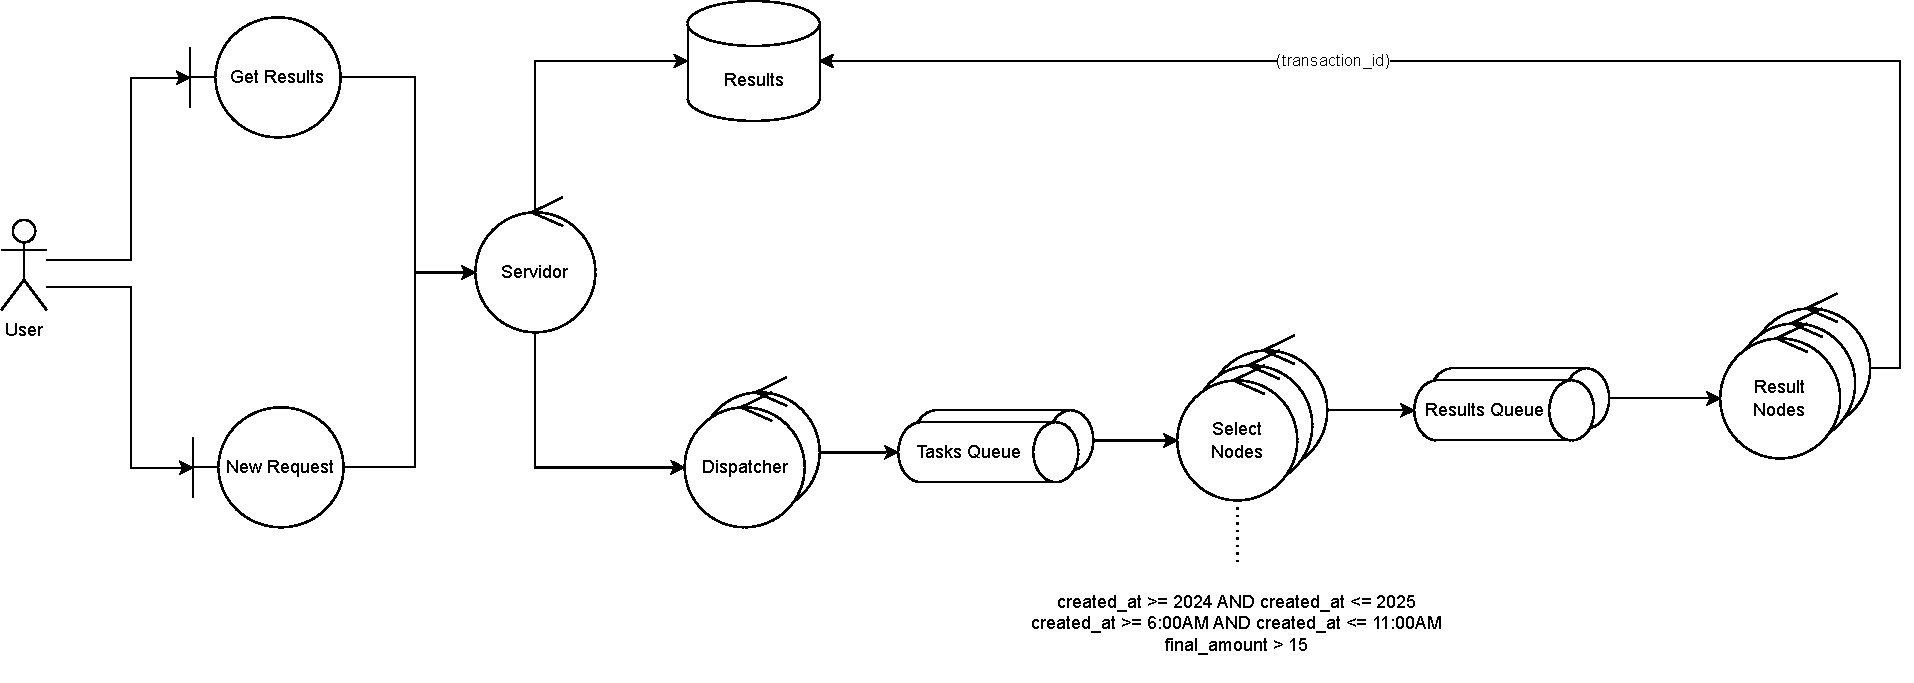
\includegraphics[width=1\textwidth]{img/robustez_1.pdf}
    \caption{Diagrama de robustez consulta 1°}
\end{figure}

En la consulta 2, TODO

\begin{figure}[H]
    \centering
    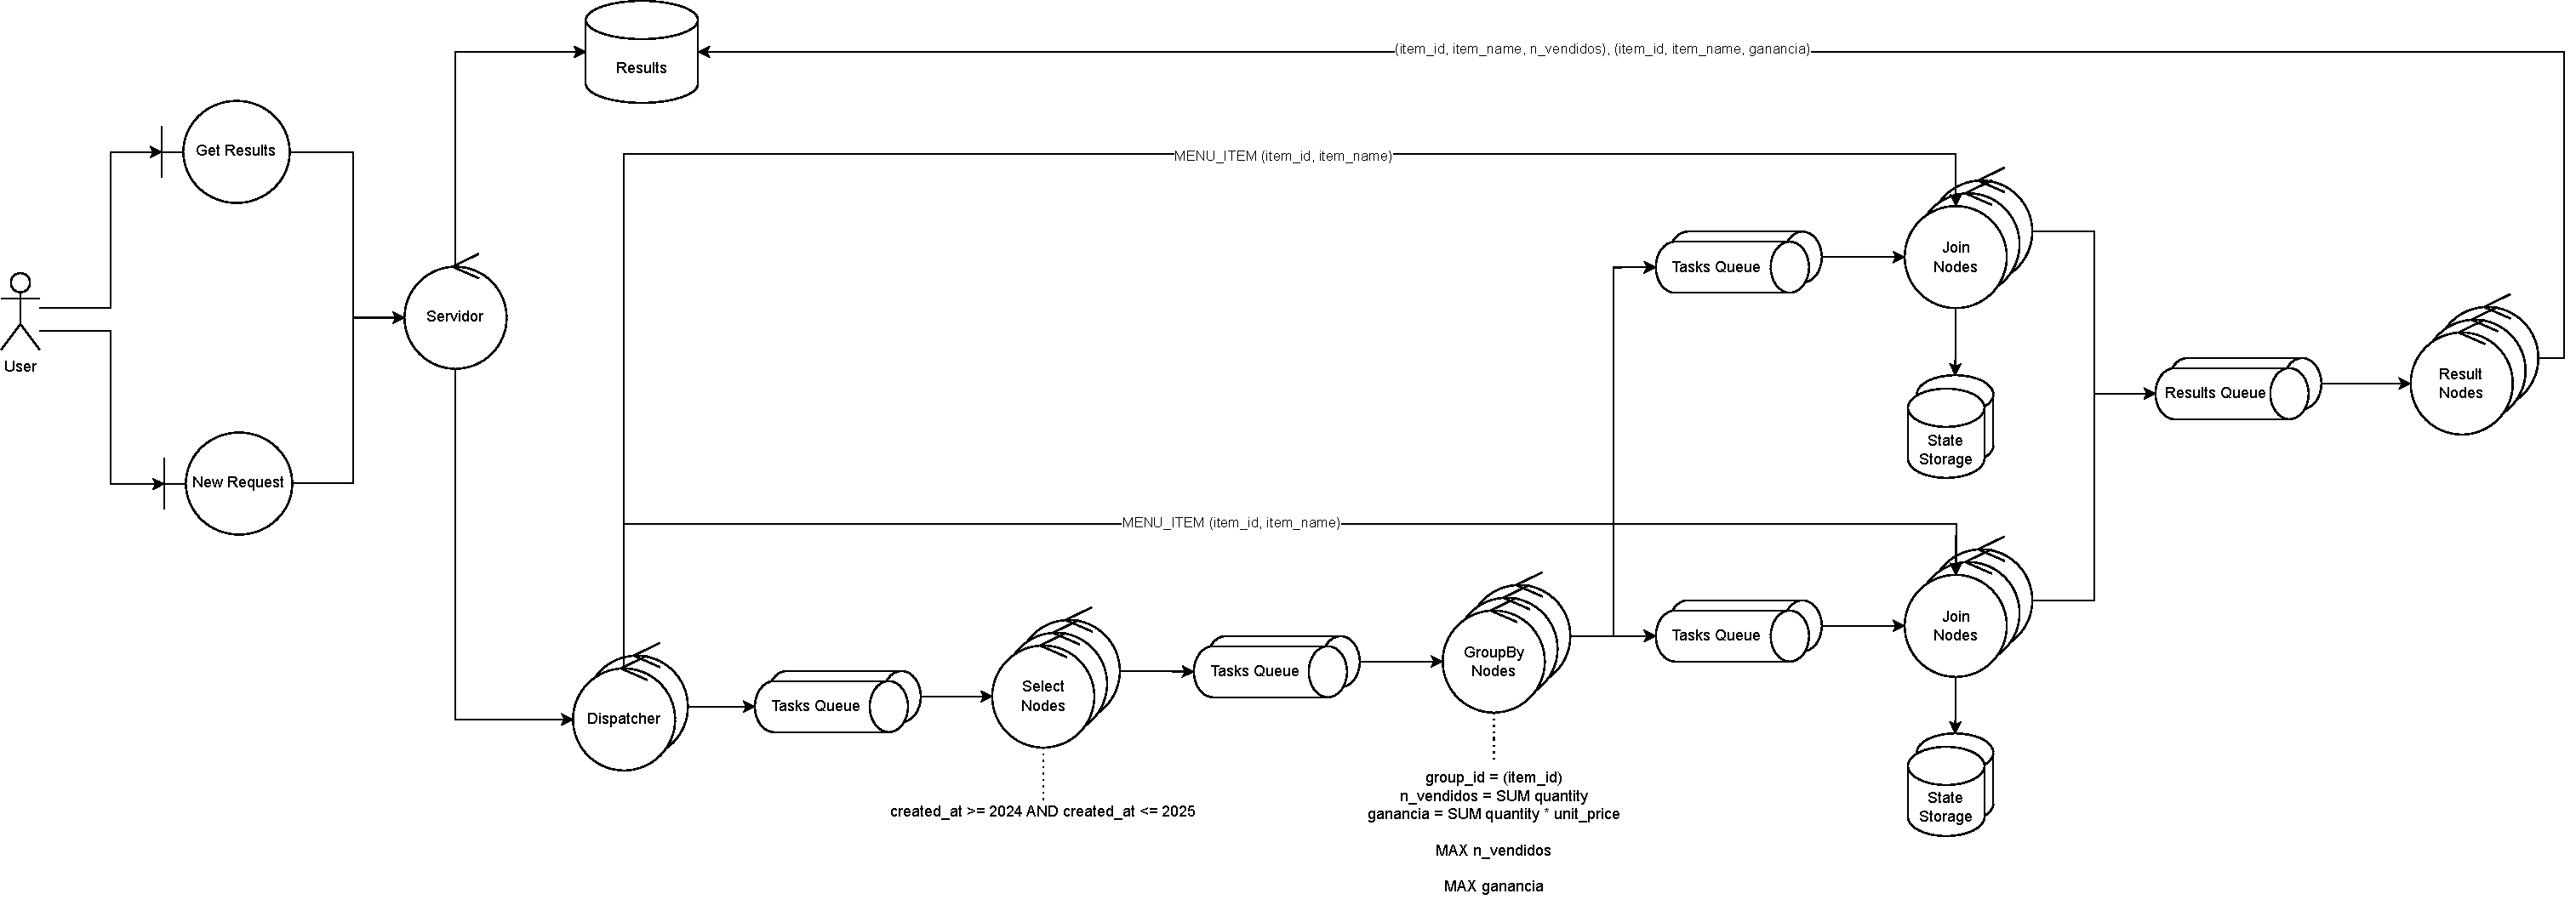
\includegraphics[width=1\textwidth]{img/robustez_2.pdf}
    \caption{Diagrama de robustez consulta 2°}
\end{figure}

En la consulta 3, TODO

\begin{figure}[H]
    \centering
    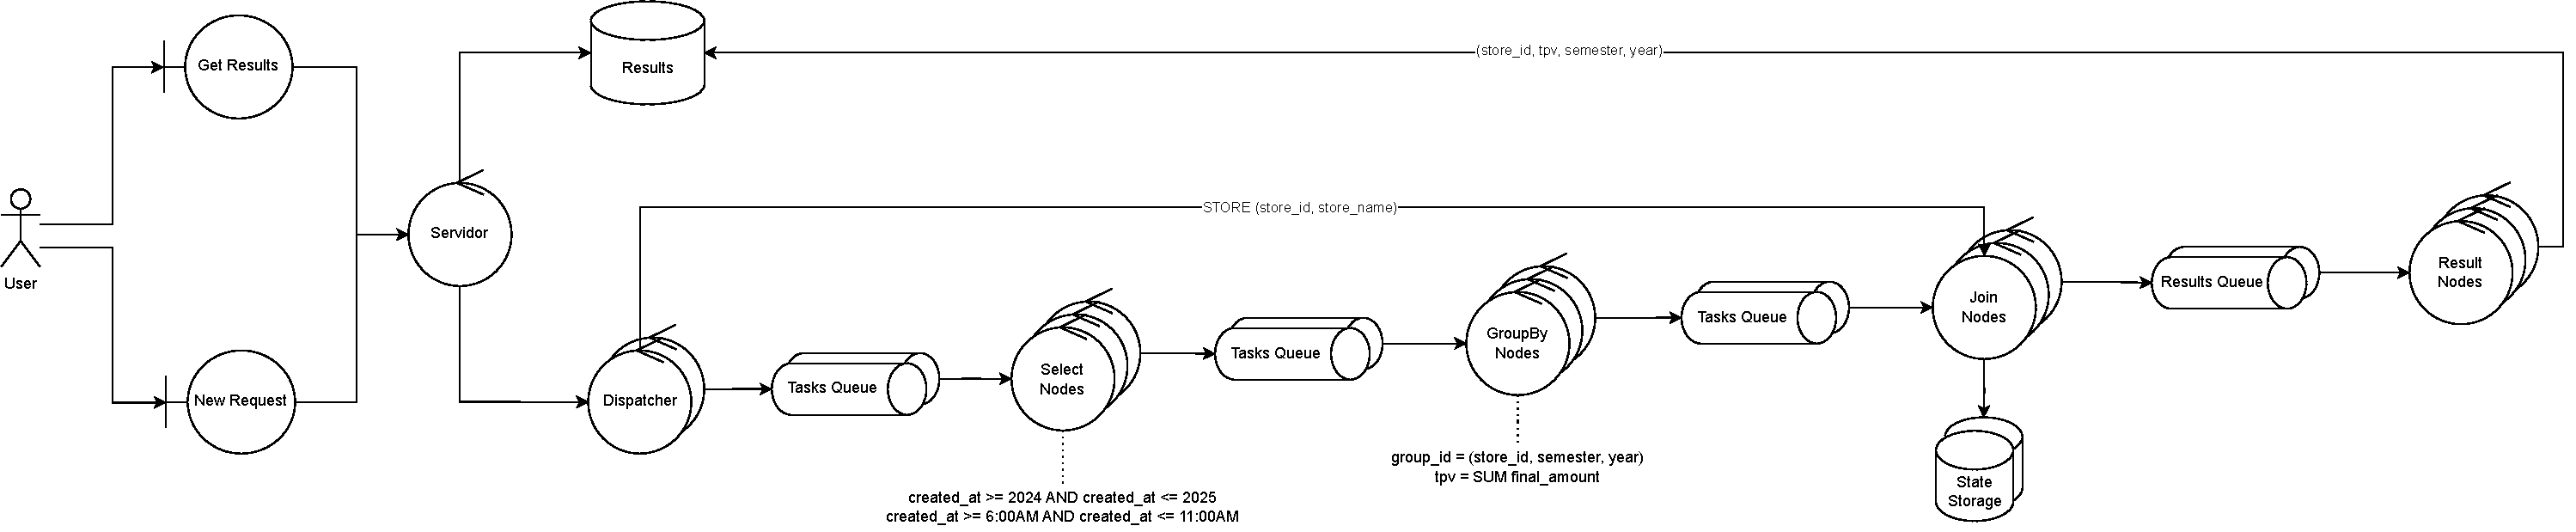
\includegraphics[width=1\textwidth]{img/robustez_3.pdf}
    \caption{Diagrama de robustez consulta 3°}
\end{figure}

En la consulta 4, TODO

\begin{figure}[H]
    \centering
    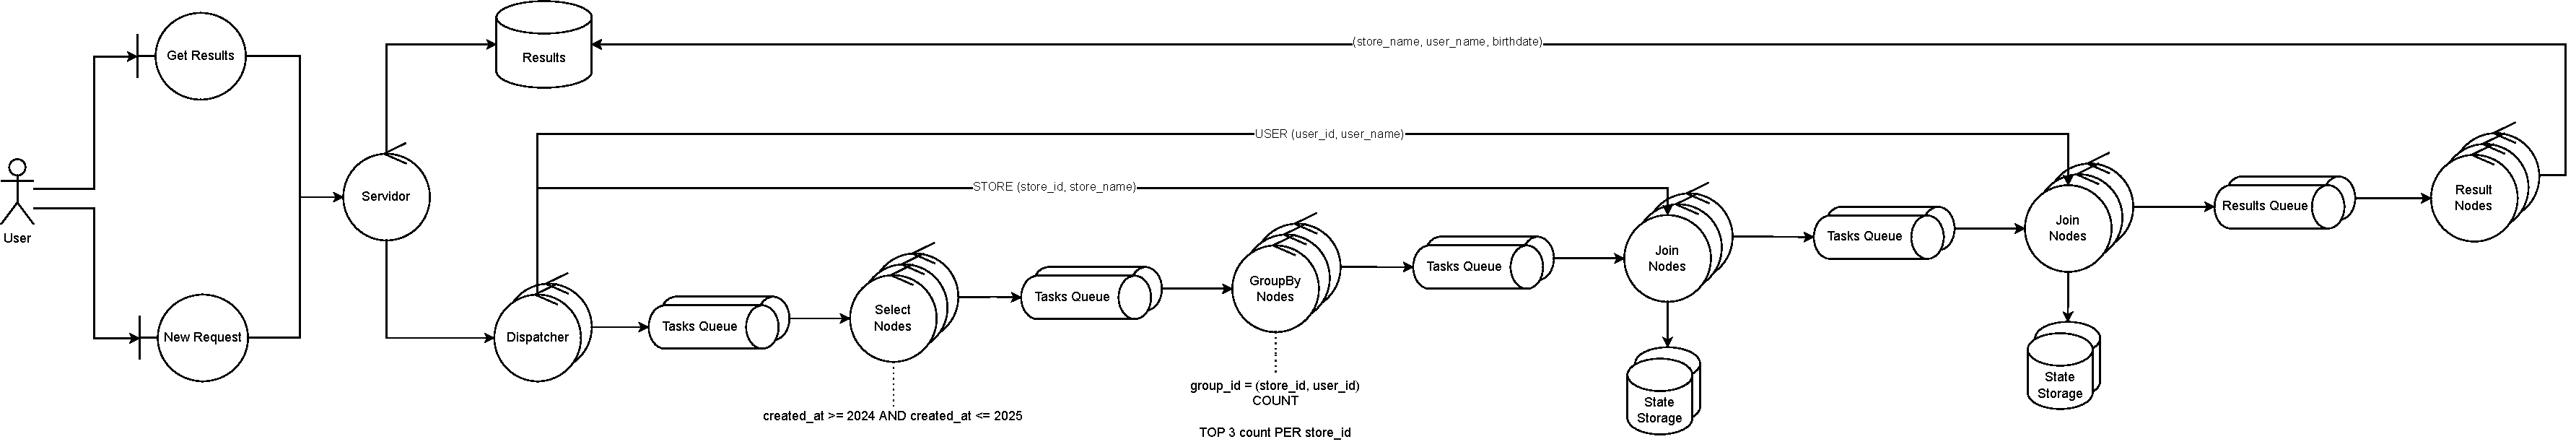
\includegraphics[width=1\textwidth]{img/robustez_4.pdf}
    \caption{Diagrama de robustez consulta 4°}
\end{figure}

\subsection{Despliegue}

TODO select queue y select node en la misma entidad

\begin{figure}[H]
    \centering
    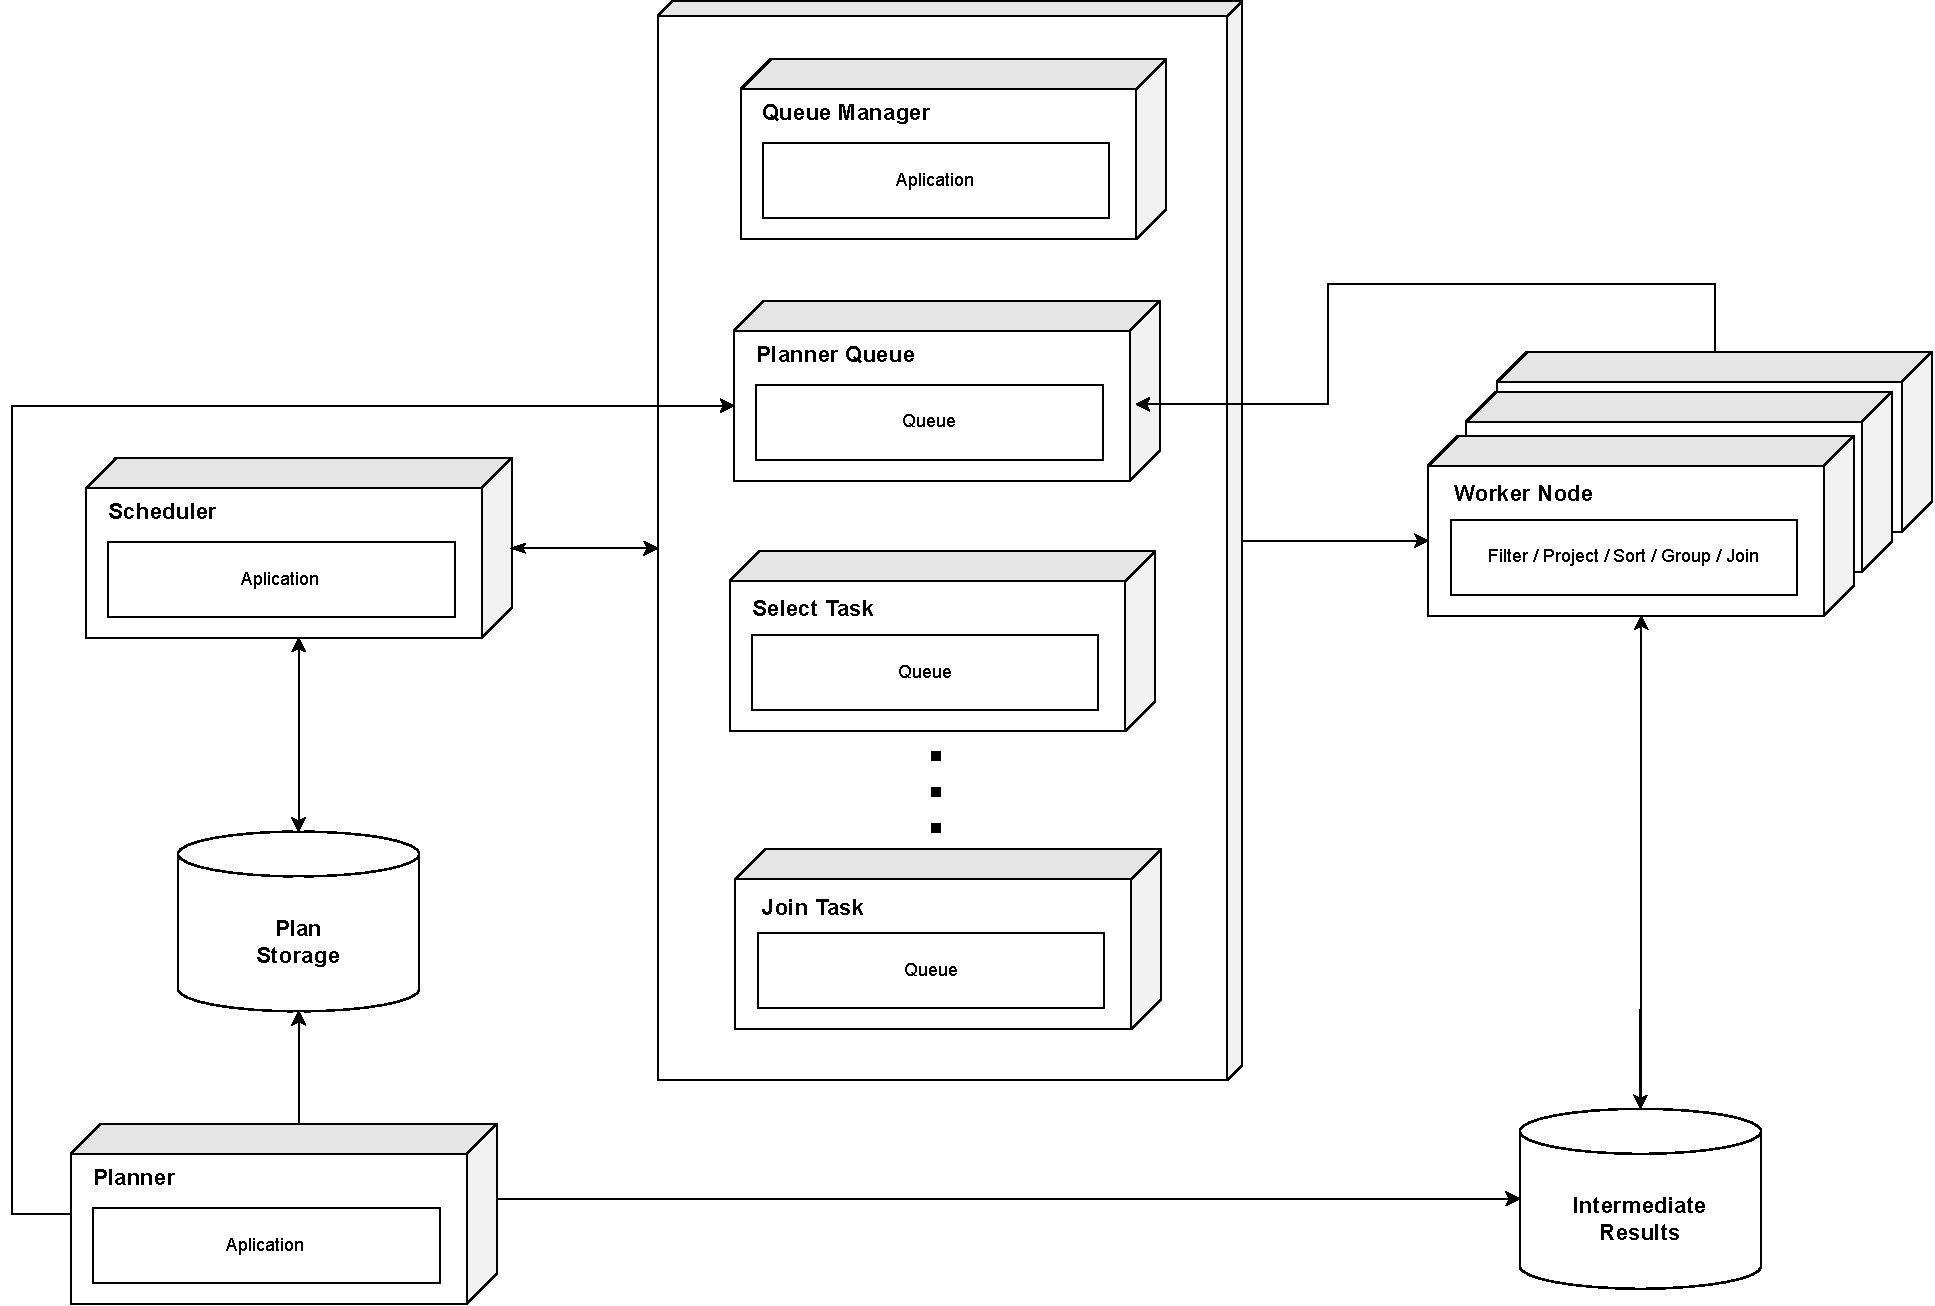
\includegraphics[width=1\textwidth]{img/despliegue.pdf}
    \caption{Diagrama de despliegue}
\end{figure}